\documentclass[dvipdfmx]{jsarticle}
\setcounter{section}{4}
\setcounter{subsection}{0}
\usepackage{xr}
\externaldocument{2.1.2}
\usepackage{amsmath,amsfonts,amssymb,array,comment,mathtools,url,docmute}
\usepackage{longtable,booktabs,dcolumn,tabularx,mathtools,multirow,colortbl,xcolor}
\usepackage[dvipdfmx]{graphics}
\usepackage{bmpsize}
\usepackage{amsthm}
\usepackage{enumitem}
\setlistdepth{20}
\renewlist{itemize}{itemize}{20}
\setlist[itemize]{label=•}
\renewlist{enumerate}{enumerate}{20}
\setlist[enumerate]{label=\arabic*.}
\setcounter{MaxMatrixCols}{20}
\setcounter{tocdepth}{3}
\newcommand{\rotin}{\text{\rotatebox[origin=c]{90}{$\in $}}}
\newcommand{\amap}[6]{\text{\raisebox{-0.7cm}{\begin{tikzpicture} 
  \node (a) at (0, 1) {$\textstyle{#2}$};
  \node (b) at (#6, 1) {$\textstyle{#3}$};
  \node (c) at (0, 0) {$\textstyle{#4}$};
  \node (d) at (#6, 0) {$\textstyle{#5}$};
  \node (x) at (0, 0.5) {$\rotin $};
  \node (x) at (#6, 0.5) {$\rotin $};
  \draw[->] (a) to node[xshift=0pt, yshift=7pt] {$\textstyle{\scriptstyle{#1}}$} (b);
  \draw[|->] (c) to node[xshift=0pt, yshift=7pt] {$\textstyle{\scriptstyle{#1}}$} (d);
\end{tikzpicture}}}}
\newcommand{\twomaps}[9]{\text{\raisebox{-0.7cm}{\begin{tikzpicture} 
  \node (a) at (0, 1) {$\textstyle{#3}$};
  \node (b) at (#9, 1) {$\textstyle{#4}$};
  \node (c) at (#9+#9, 1) {$\textstyle{#5}$};
  \node (d) at (0, 0) {$\textstyle{#6}$};
  \node (e) at (#9, 0) {$\textstyle{#7}$};
  \node (f) at (#9+#9, 0) {$\textstyle{#8}$};
  \node (x) at (0, 0.5) {$\rotin $};
  \node (x) at (#9, 0.5) {$\rotin $};
  \node (x) at (#9+#9, 0.5) {$\rotin $};
  \draw[->] (a) to node[xshift=0pt, yshift=7pt] {$\textstyle{\scriptstyle{#1}}$} (b);
  \draw[|->] (d) to node[xshift=0pt, yshift=7pt] {$\textstyle{\scriptstyle{#2}}$} (e);
  \draw[->] (b) to node[xshift=0pt, yshift=7pt] {$\textstyle{\scriptstyle{#1}}$} (c);
  \draw[|->] (e) to node[xshift=0pt, yshift=7pt] {$\textstyle{\scriptstyle{#2}}$} (f);
\end{tikzpicture}}}}
\renewcommand{\thesection}{第\arabic{section}部}
\renewcommand{\thesubsection}{\arabic{section}.\arabic{subsection}}
\renewcommand{\thesubsubsection}{\arabic{section}.\arabic{subsection}.\arabic{subsubsection}}
\everymath{\displaystyle}
\allowdisplaybreaks[4]
\usepackage{vtable}
\theoremstyle{definition}
\newtheorem{thm}{定理}[subsection]
\newtheorem*{thm*}{定理}
\newtheorem{dfn}{定義}[subsection]
\newtheorem*{dfn*}{定義}
\newtheorem{axs}[dfn]{公理}
\newtheorem*{axs*}{公理}
\renewcommand{\headfont}{\bfseries}
\makeatletter
  \renewcommand{\section}{%
    \@startsection{section}{1}{\z@}%
    {\Cvs}{\Cvs}%
    {\normalfont\huge\headfont\raggedright}}
\makeatother
\makeatletter
  \renewcommand{\subsection}{%
    \@startsection{subsection}{2}{\z@}%
    {0.5\Cvs}{0.5\Cvs}%
    {\normalfont\LARGE\headfont\raggedright}}
\makeatother
\makeatletter
  \renewcommand{\subsubsection}{%
    \@startsection{subsubsection}{3}{\z@}%
    {0.4\Cvs}{0.4\Cvs}%
    {\normalfont\Large\headfont\raggedright}}
\makeatother
\makeatletter
\renewenvironment{proof}[1][\proofname]{\par
  \pushQED{\qed}%
  \normalfont \topsep6\p@\@plus6\p@\relax
  \trivlist
  \item\relax
  {
  #1\@addpunct{.}}\hspace\labelsep\ignorespaces
}{%
  \popQED\endtrivlist\@endpefalse
}
\makeatother
\renewcommand{\proofname}{\textbf{証明}}
\usepackage{tikz,graphics}
\usepackage[dvipdfmx]{hyperref}
\usepackage{pxjahyper}
\hypersetup{
 setpagesize=false,
 bookmarks=true,
 bookmarksdepth=tocdepth,
 bookmarksnumbered=true,
 colorlinks=false,
 pdftitle={},
 pdfsubject={},
 pdfauthor={},
 pdfkeywords={}}
\begin{document}
%\hypertarget{ux5546vectorux7a7aux9593}{%
\subsection{商vector空間}%\label{ux5546vectorux7a7aux9593}}\par
%\hypertarget{ux5546ux96c6ux5408}{%
\begin{comment}
\subsubsection{商集合}%\label{ux5546ux96c6ux5408}}
\begin{dfn}
集合たち$A$、$B$が与えられたとする。このとき、$R = (A,B,G):A \multimap B$なる対応$R$を考えると、その値域$V\left( R| \left\{ a \right\} \right)$が空集合でないとき、対応の定義より次式が成り立つような元$b$がその集合$B$に存在する。
\begin{align*}
b \in V\left( R \middle| \left\{ a \right\} \right) \subseteq B
\end{align*}
このことを$aRb$と書きその対応$R$をその集合$A$からその集合$B$への関係といい、これのgraph$G$をその関係$R$のgraphといい$G(R)$とも書く。特に、$A = B$のとき、その関係$R$はその集合$A$における関係という。
\end{dfn}\par
例えば、等号$=$、必要十分条件$\Leftrightarrow$などが挙げられる。
\begin{axs}{同値関係の公理}
次のことを満たすような関係$R:A \multimap A$をその集合$A$における同値関係という。
\begin{itemize}
\item
  その関係$R$は反射的である、即ち、$\forall a \in A$に対し、$aRa$が成り立つ。
\item
  その関係$R$は対称的である、即ち、$\forall a,b \in A$に対し、$aRb$が成り立つならそのときに限り、$bRa$が成り立つ。
\item
  その関係$R$は推移的である、即ち、$\forall a,b,c \in A$に対し、$aRb$かつ$bRc$が成り立つなら、$aRc$が成り立つ。
\end{itemize}
\end{axs}
\begin{dfn}
集合$A$における同値関係$R$が与えられたとき、$aRb$なるその集合$A$の2つの元々$a$、$b$はその同値関係$R$に関して同値であるという。
\end{dfn}
\begin{thm}\label{2.4.1.1}
集合$A$の2つの同値関係たち$R$、$S$が与えられたとき、$\forall a,b \in A$に対し、$aRb$ならそのときに限り、$aSb$が成り立つことが成り立つならそのときに限り、$R = S$が成り立つ。\par
なお、以下、定理\ref{2.4.1.7}まで証明を割愛させていただく。詳しくは集合論のほうに参照されたい\footnote{だって、量がすごいんだもん…(*\_*)}。
\end{thm}
\begin{dfn}
その集合$\mathfrak{M}$に属する集合たち全体の和集合$\bigcup_{} \mathfrak{M}$のうち、$\forall A,B \in \mathfrak{M}$に対し、$A \cap B = \emptyset$が成り立つようなものをその集合$\mathfrak{M}$に属する集合たち全体の直和、非交和などといい$\bigsqcup_{A \in \mathfrak{M}} A$、$\bigsqcup_{} \mathfrak{M}$、$\bigsqcup_{\mathfrak{M}} $などと書く。
\end{dfn}
\begin{dfn}
ここで、その集合$\mathfrak{M}$はその集合$\bigsqcup_{} \mathfrak{M}$の直和分割である、その集合$\bigsqcup_{} \mathfrak{M}$はその集合$\mathfrak{M}$に属する集合の直和であるなどともいう。
\end{dfn}
\begin{thm}\label{2.4.1.2}
$\forall a \in \bigsqcup_{} \mathfrak{M}$に対し、$a \in A$なる集合$A$がその集合$\mathfrak{M}$に一意的に存在する。
\end{thm}
\begin{thm}\label{2.4.1.3}
その集合$\bigsqcup_{} \mathfrak{M}$の元々$a$、$b$に対し、次式のように論理式$aR_{\mathfrak{M}}b$が定義されると、
\begin{align*}
aR_{\mathfrak{M}}b \Leftrightarrow a \in A \land b \in B \land A,B \in \mathfrak{M \land}A = B
\end{align*}
その集合$\bigsqcup_{} \mathfrak{M}$における関係$R_{\mathfrak{M}}$が得られこれは同値関係となる。
\end{thm}
\begin{dfn}
この関係$R_{\mathfrak{M}}$をその直和分割$\mathfrak{M}$に付随する同値関係という。
\end{dfn}\par
このことは次のようにして考えられればわかりやすかろう。
\begin{center}
  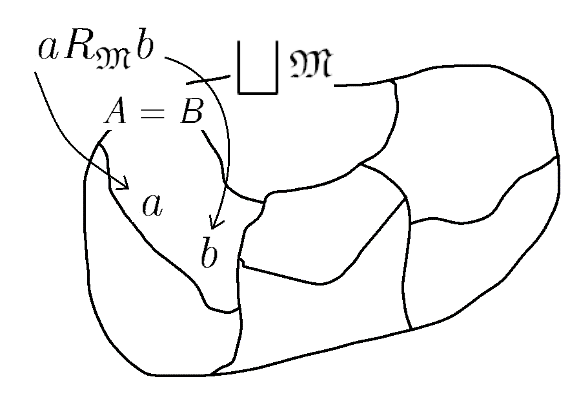
\includegraphics[width=160pt]{1.2.5.a.png}
\end{center}
\begin{dfn}
集合$A$の1つの同値関係$R$が与えられたとする。このとき、次式のような集合$C_{R}(a)$が定義されよう。
\begin{align*}
C_{R}(a) = \left\{ c \in A \middle| aRc \right\} \subseteq A
\end{align*}
この集合$C_{R}(a)$をその同値関係$R$によるその元$a$の同値類、または単に、類などといい$[ a]_{R}$、$\overline{a}$などとも書く。
\end{dfn}\par
このことは次のようにして考えられればわかりやすかろう。
\begin{center}
  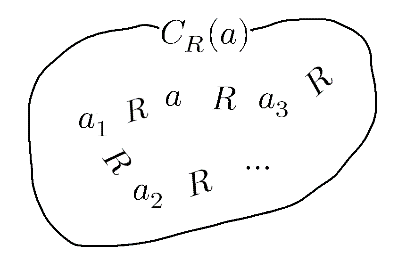
\includegraphics[width=160pt]{1.2.5.b.png}
\end{center}
\begin{thm}\label{2.4.1.4}
次のことが成り立つ。
\begin{itemize}
\item
  $\forall a \in A$に対し、$a \in C_{R}(a)$が成り立つ。
\item
  $\forall a,b \in A$に対し、$aRb$が成り立つならそのときに限り、$C_{R}(a) = C_{R}(b)$が成り立つ。
\item
  $\forall a,b \in A$に対し、$C_{R}(a) \neq C_{R}(b)$が成り立つなら、$C_{R}(a) \cap C_{R}(b) = \emptyset$が成り立つ。
\end{itemize}
\end{thm}
\begin{thm}\label{2.4.1.5}
集合$A$の1つの同値関係$R$が与えられたとする。次式のようにその同値関係$R$によるその元$a$の同値類全体の集合$\mathfrak{M}$が定義されると、
\begin{align*}
\mathfrak{M}=\left\{ C_{R}(a)\in \mathfrak{P}(A) \middle| C_{R}(a) = \left\{ c \in A \middle| aRc \right\} \right\}
\end{align*}
その集合$\mathfrak{M}$はその集合$A$の直和分割でこれに付随する同値関係$R_{\mathfrak{M}}$はその同値関係$R$に等しい。
\end{thm}\par
このことは次のようにして考えられればわかりやすかろう。
\begin{center}
    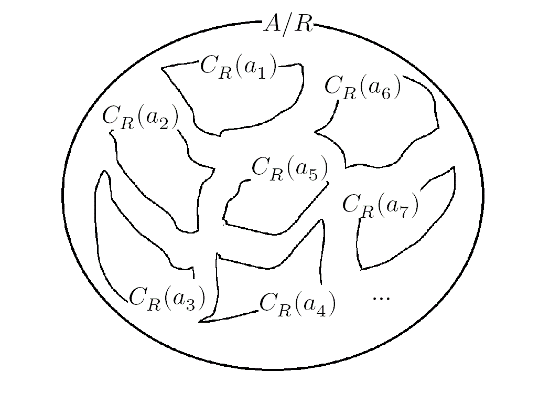
\includegraphics[width=160pt]{1.2.5.c.png}
\end{center}
\begin{dfn}
このようにして、その同値関係$R$からその集合$\mathfrak{M}$が定義されること、即ち、その集合$A$がその同値関係$R$によって得られる同値類たちの直和$\bigsqcup_{} \mathfrak{M}$とみなすことをその集合$A$のその同値関係$R$による類別、分類といいその集合$\mathfrak{M}$をその集合$A$のその同値関係による商集合といい$A/R$などと書く。
\end{dfn}
\begin{thm}\label{2.4.1.6}
ここで、写像$f:A \rightarrow B$が与えられたとする。このとき、その集合$A$の元々$a$、$b$に対し、次式のように論理式$aR(f)b$が定義されると、
\begin{align*}
aR(f)b \Leftrightarrow a,b \in A \land f(a) = f(b)
\end{align*}
その集合$A$における関係$R(f)$が得られこれは同値関係となる。
\end{thm}
\begin{dfn}
この関係$R(f)$をその写像$f$に付随する同値関係、その写像$f$の同値核などという。
\end{dfn}
\begin{thm}\label{2.4.1.7}
集合$A$の1つの同値関係$R$が与えられたとする。次式のように写像$C_{R}$が定義されるとき、
\begin{align*}
C_{R}:A \rightarrow A/R;a \mapsto C_{R}(a)
\end{align*}
その写像$C_{R}$は全射でありこれに付随する同値関係$R\left( C_{R} \right)$はその同値関係$R$に等しい。
\end{thm}
\begin{dfn}
このような写像$C_{R}$をその集合$A$からその集合$A/R$への標準的全射、自然な全射、商写像などという。
\end{dfn}
\end{comment}
%\hypertarget{ux5546vectorux7a7aux9593-1}{%
\subsubsection{商vector空間}%\label{ux5546vectorux7a7aux9593-1}}
\begin{dfn}
体$K$上のvector空間$V$の部分空間$W$が与えられたとき、$\mathbf{v},\mathbf{w} \in V$に対し、$\mathbf{v} - \mathbf{w} \in W$が成り立つことを$\mathbf{v} \equiv \mathbf{w}\ \mathrm{mod}W$と書くことにする。
\end{dfn}
\begin{thm}\label{2.4.1.8}
体$K$上のvector空間$V$の部分空間$W$が与えられたとき、上記の関係$\equiv \ \mathrm{mod}W$は同値関係である。
\end{thm}
\begin{proof}
体$K$上のvector空間$V$の部分空間$W$が与えられたとき、$\forall\mathbf{v} \in V$に対し、$\mathbf{0} = \mathbf{v} - \mathbf{v} \in W$が成り立つので、$\mathbf{v} \equiv \mathbf{v}\ \mathrm{mod}W$が成り立つ。$\forall\mathbf{v},\mathbf{w} \in W$に対し、$\mathbf{v} \equiv \mathbf{w}\ \mathrm{mod}W$が成り立つなら、$\mathbf{v} - \mathbf{w} \in W$が成り立ち、したがって、$\mathbf{w} - \mathbf{v} = - \mathbf{v} + \mathbf{w} = - \left( \mathbf{v} - \mathbf{w} \right) \in W$が成り立つので、$\mathbf{w} \equiv \mathbf{v}\ \mathrm{mod}W$が成り立つ。最後に、$\forall\mathbf{u},\mathbf{v},\mathbf{w} \in V$に対し、$\mathbf{u} \equiv \mathbf{v}\ \mathrm{mod}W$かつ$\mathbf{v} \equiv \mathbf{w}\ \mathrm{mod}W$が成り立つなら、$\mathbf{u} - \mathbf{v},\mathbf{v} - \mathbf{w} \in W$が成り立つので、$\mathbf{u} - \mathbf{w} = \mathbf{u} - \mathbf{v} + \mathbf{v} - \mathbf{w} = \left( \mathbf{u} - \mathbf{v} \right) + \left( \mathbf{v} - \mathbf{w} \right) \in W$が成り立つ。したがって、$\mathbf{u} \equiv \mathbf{w}\ \mathrm{mod}W$が成り立つ。以上より、その関係$\equiv \ \mathrm{mod}W$は同値関係である。
\end{proof}
\begin{thm}\label{2.4.1.9}
体$K$上のvector空間$V$の部分空間$W$が与えられたとき、$\forall k,l \in K$に対し、$k \neq 0$または$l \neq 0$が成り立つなら、$kW + lW = W$が成り立つ。
\end{thm}
\begin{proof}
体$K$上のvector空間$V$の部分空間$W$が与えられたとき、$\forall k,l \in K\forall\mathbf{v},\mathbf{w} \in W$に対し、$k \neq 0$または$l \neq 0$が成り立つなら、$k\mathbf{v} + l\mathbf{w} \in kW + lW$が成り立ち、これより明らかに、$k\mathbf{v} + l\mathbf{w} \in W$も成り立つので、$kW + lW \subseteq W$が成り立つ。一方で、$\forall\mathbf{v} \in W$に対し、$k \neq 0$としても一般性は失われなく、このとき、$\frac{1}{k}\mathbf{v} \in W$が成り立つので、$\mathbf{v} = k\frac{1}{k}\mathbf{v} + l\mathbf{0} \in kW + lW$が成り立つ。以上より、$kW + lW = W$が成り立つ。
\end{proof}
\begin{thm}\label{2.4.1.10}
体$K$上のvector空間$V$の部分空間$W$が与えられたとき、上記の議論により商集合${V}/{\equiv \ \mathrm{mod}W}$が定義される。このとき、$\forall C_{\equiv \ \mathrm{mod}W}\left( \mathbf{v} \right) \in {V}/{\equiv \ \mathrm{mod}W}$に対し、$C_{\equiv \ \mathrm{mod}W}\left( \mathbf{v} \right) = \mathbf{v} + W$が成り立つ。
\end{thm}
\begin{proof}
体$K$上のvector空間$V$の部分空間$W$が与えられたとき、上記の議論により商集合${V}/{\equiv \ \mathrm{mod}W}$が定義される。このとき、$\forall C_{\equiv \ \mathrm{mod}W}\left( \mathbf{v} \right) \in {V}/{\equiv \ \mathrm{mod}W}\forall\mathbf{w} \in C_{\equiv \ \mathrm{mod}W}\left( \mathbf{v} \right)$に対し、$\mathbf{v} \equiv \mathbf{w}\ \mathrm{mod}W$が成り立つので、$\mathbf{v} - \mathbf{w} \in W$が成り立つ。ここで、$- \mathbf{u} = \mathbf{v} - \mathbf{w}$とおかれると、$\mathbf{w} = \mathbf{v} + \mathbf{u}$が成り立つかつ、$\mathbf{u}, - \mathbf{u} \in W$が成り立つので、$\mathbf{w} \in \mathbf{v} + W$が成り立つ。逆に、$\forall\mathbf{v} + \mathbf{w} \in \mathbf{v} + W$に対し、$\mathbf{w} \in W$が成り立つので、$\mathbf{w} = \mathbf{v} + \mathbf{w} - \mathbf{v} = \left( \mathbf{v} + \mathbf{w} \right) - \mathbf{v} \in W$となり、したがって、$\mathbf{v} + \mathbf{w} \equiv \mathbf{v}\ \mathrm{mod}W$が成り立ち、これにより、$\mathbf{v} + \mathbf{w} \in C_{\equiv \ \mathrm{mod}W}\left( \mathbf{v} \right)$が成り立つ。以上より、$C_{\equiv \ \mathrm{mod}W}\left( \mathbf{v} \right) = \mathbf{v} + W$が成り立つ。
\end{proof}
\begin{thm}\label{2.4.1.11}
体$K$上のvector空間$V$の部分空間$W$が与えられたとき、$W = C_{\equiv \ \mathrm{mod}W}\left( \mathbf{0} \right) \in {V}/{\equiv \ \mathrm{mod}W}$が成り立つ。
\end{thm}
\begin{proof} $W = \mathbf{0} + W$が成り立つことによる。
\end{proof}
\begin{thm}\label{2.4.1.12}
体$K$上のvector空間$V$の部分空間$W$が与えられたとき、$\forall\mathbf{v},\mathbf{w} \in V$に対し、$\mathbf{v} \equiv \mathbf{w}\ \mathrm{mod}W$が成り立つなら、$\mathbf{v} + W = \mathbf{w} + W$が成り立ち、そうでないなら、$\mathbf{v} + W \cap \mathbf{w} + W = \emptyset$が成り立つ。
\end{thm}
\begin{proof}
体$K$上のvector空間$V$の部分空間$W$が与えられたとき、$\forall\mathbf{v},\mathbf{w} \in V$に対し、$\mathbf{v} \equiv \mathbf{w}\ \mathrm{mod}W$が成り立つなら、$\mathbf{v} \in C_{\equiv \ \mathrm{mod}W}\left( \mathbf{w} \right) = \mathbf{w} + W$が成り立つので、$\forall\mathbf{v} + \mathbf{u} \in \mathbf{v} + W$に対し、あるその部分空間$W$の元$\mathbf{u}'$が存在して$\mathbf{v} = \mathbf{w} + \mathbf{u}'$が成り立ち、したがって、$\mathbf{v} + \mathbf{u} = \mathbf{w} + \left( \mathbf{u}' + \mathbf{u} \right) \in \mathbf{w} + W$が成り立つ。ゆえに、$\mathbf{v} + W \subseteq \mathbf{w} + W$が成り立つ。同様にして、$\mathbf{v} + W \supseteq \mathbf{w} + W$が成り立つので、$\mathbf{v} + W = \mathbf{w} + W$が成り立つ。\par
$\mathbf{v} + W \cap \mathbf{w} + W \neq \emptyset$が成り立つなら、$\mathbf{u} \in \mathbf{v} + W \cap \mathbf{w} + W$なるその集合$\mathbf{v} + W \cap \mathbf{w} + W$の元$\mathbf{u}$が存在して、$\exists\mathbf{u}',\mathbf{u}'' \in W$に対し、$\mathbf{u} = \mathbf{v} + \mathbf{u}' = \mathbf{w} + \mathbf{u}''$が成り立つので、$\mathbf{u} - \mathbf{v},\mathbf{u} - \mathbf{w} \in W$が成り立つ。このとき、$\mathbf{u} \equiv \mathbf{v}\ \mathrm{mod}W$かつ$\mathbf{u} \equiv \mathbf{w}\ \mathrm{mod}W$が成り立つので、$\mathbf{v} \equiv \mathbf{w}\ \mathrm{mod}W$が成り立つ。対偶律より$\mathbf{v} \equiv \mathbf{w}\ \mathrm{mod}W$が成り立たないなら、$\mathbf{v} + W \cap \mathbf{w} + W = \emptyset$が成り立つ。
\end{proof}
\begin{thm}\label{2.4.1.13}
体$K$上のvector空間$V$の部分空間$W$が与えられたとき、上記の議論により商集合${V}/{\equiv \ \mathrm{mod}W}$が定義される。このとき、$\forall k \in K\forall C_{\equiv \ \mathrm{mod}W}\left( \mathbf{v} \right) \in {V}/{\equiv \ \mathrm{mod}W}$に対し、次式のように定義されると、
\begin{align*}
kC_{\equiv \ \mathrm{mod}W}\left( \mathbf{v} \right) = C_{\equiv \ \mathrm{mod}W}\left( k\mathbf{v} \right)
\end{align*}
その集合${V}/{\equiv \ \mathrm{mod}W}$は体$K$上のvector空間をなす。
\end{thm}
\begin{dfn}
このようにして構成されたvector空間${V}/{\equiv \ \mathrm{mod}W}$をそのvector空間$V$のその部分空間$W$による商vector空間、商線形空間、商空間といい、${V}/{W}$と書く。
\end{dfn}
\begin{proof}
体$K$上のvector空間$V$の部分空間$W$が与えられたとき、上記の議論により商集合${V}/{\equiv \ \mathrm{mod}W}$が定義される。このとき、$\forall k \in K\forall C_{\equiv \ \mathrm{mod}W}\left( \mathbf{v} \right) \in {V}/{\equiv \ \mathrm{mod}W}$に対し、次式のように定義されると、
\begin{align*}
kC_{\equiv \ \mathrm{mod}W}\left( \mathbf{v} \right) = C_{\equiv \ \mathrm{mod}W}\left( k\mathbf{v} \right)
\end{align*}
$\forall\mathbf{u},\mathbf{v},\mathbf{w} \in V$に対し、次のようになることから、
\begin{align*}
\left( C_{\equiv \ \mathrm{mod}W}\left( \mathbf{u} \right) + C_{\equiv \ \mathrm{mod}W}\left( \mathbf{v} \right) \right) + C_{\equiv \ \mathrm{mod}W}\left( \mathbf{w} \right) &= \left( \mathbf{u} + W + \mathbf{v} + W \right) + \mathbf{w} + W\\
&= \mathbf{u} + W + \left( \mathbf{v} + W + \mathbf{w} + W \right)\\
&= C_{\equiv \ \mathrm{mod}W}\left( \mathbf{u} \right) + \left( C_{\equiv \ \mathrm{mod}W}\left( \mathbf{v} \right) + C_{\equiv \ \mathrm{mod}W}\left( \mathbf{w} \right) \right)\\
C_{\equiv \ \mathrm{mod}W}\left( \mathbf{v} \right) + C_{\equiv \ \mathrm{mod}W}\left( \mathbf{0} \right) &= \mathbf{v} + W + \mathbf{0} + W = \mathbf{v} + W + W\\
&= \mathbf{v} + W = C_{\equiv \ \mathrm{mod}W}\left( \mathbf{v} \right)\\
C_{\equiv \ \mathrm{mod}W}\left( \mathbf{v} \right) + C_{\equiv \ \mathrm{mod}W}\left( - \mathbf{v} \right) &= \mathbf{v} + W - \mathbf{v} + W = \mathbf{v} - \mathbf{v} + W + W\\
&= \mathbf{0} + W = C_{\equiv \ \mathrm{mod}W}\left( \mathbf{0} \right)\\
C_{\equiv \ \mathrm{mod}W}\left( \mathbf{v} \right) + C_{\equiv \ \mathrm{mod}W}\left( \mathbf{w} \right) &= \mathbf{v} + W + \mathbf{w} + W\\
&= \mathbf{w} + W + \mathbf{v} + W\\
&= C_{\equiv \ \mathrm{mod}W}\left( \mathbf{w} \right) + C_{\equiv \ \mathrm{mod}W}\left( \mathbf{v} \right)
\end{align*}
その組$\left( {V}/{\equiv \ \mathrm{mod}W}, + \right)$は可換群をなす。\par
このとき、$\forall k,l \in K$に対し、次のようになることから、
\begin{align*}
k\left( C_{\equiv \ \mathrm{mod}W}\left( \mathbf{v} \right) + C_{\equiv \ \mathrm{mod}W}\left( \mathbf{w} \right) \right) &= k\left( \mathbf{v} + W + \mathbf{w} + W \right)\\
&= k\left( \mathbf{v} + \mathbf{w} + W \right)\\
&= kC_{\equiv \ \mathrm{mod}W}\left( \mathbf{v} + \mathbf{w} \right)\\
&= C_{\equiv \ \mathrm{mod}W}\left( k\left( \mathbf{v} + \mathbf{w} \right) \right)\\
&= C_{\equiv \ \mathrm{mod}W}\left( k\mathbf{v} + k\mathbf{w} \right)\\
&= k\mathbf{v} + k\mathbf{w} + W\\
&= k\mathbf{v} + W + k\mathbf{w} + W\\
&= C_{\equiv \ \mathrm{mod}W}\left( k\mathbf{v} \right) + C_{\equiv \ \mathrm{mod}W}\left( k\mathbf{w} \right)\\
&= kC_{\equiv \ \mathrm{mod}W}\left( \mathbf{v} \right) + kC_{\equiv \ \mathrm{mod}W}\left( \mathbf{w} \right)\\
(k + l)C_{\equiv \ \mathrm{mod}W}\left( \mathbf{v} \right) &= C_{\equiv \ \mathrm{mod}W}\left( (k + l)\mathbf{v} \right)\\
&= C_{\equiv \ \mathrm{mod}W}\left( k\mathbf{v} + l\mathbf{v} \right)\\
&= k\mathbf{v} + l\mathbf{v} + W\\
&= k\mathbf{v} + W + l\mathbf{v} + W\\
&= C_{\equiv \ \mathrm{mod}W}\left( k\mathbf{v} \right) + C_{\equiv \ \mathrm{mod}W}\left( l\mathbf{v} \right)\\
&= kC_{\equiv \ \mathrm{mod}W}\left( \mathbf{v} \right) + lC_{\equiv \ \mathrm{mod}W}\left( \mathbf{v} \right)\\
(kl)C_{\equiv \ \mathrm{mod}W}\left( \mathbf{v} \right) &= C_{\equiv \ \mathrm{mod}W}\left( (kl)\mathbf{v} \right)\\
&= C_{\equiv \ \mathrm{mod}W}\left( k\left( l\mathbf{v} \right) \right)\\
&= kC_{\equiv \ \mathrm{mod}W}\left( l\mathbf{v} \right)\\
1C_{\equiv \ \mathrm{mod}W}\left( \mathbf{v} \right) &= C_{\equiv \ \mathrm{mod}W}\left( 1\mathbf{v} \right)\\
&= C_{\equiv \ \mathrm{mod}W}\left( \mathbf{v} \right)
\end{align*}
その集合${V}/{\equiv \ \mathrm{mod}W}$は体$K$上のvector空間をなす。
\end{proof}
\begin{thm}\label{2.4.1.14}
体$K$上の有限次元vector空間$V$の部分空間$W$が与えられたとき、これの基底が$\left\langle \mathbf{v}_{i} \right\rangle_{i \in \varLambda_{r}}$とおかれれば、次のことは同値である。
\begin{itemize}
\item
  $i \in \varLambda_{n} \setminus \varLambda_{r}$なるvectors$\mathbf{v}_{i} + W$が線形独立である。
\item
  $i \in \varLambda_{n}$なるvectors$\mathbf{v}_{i}$が線形独立である。
\end{itemize}
\end{thm}
\begin{proof}
体$K$上の有限次元vector空間$V$の部分空間$W$が与えられたとき、これの基底が$\left\langle \mathbf{v}_{i} \right\rangle_{i \in \varLambda_{r}}$とおかれれば、$i \in \varLambda_{n} \setminus \varLambda_{r}$なるvectors$\mathbf{v}_{i} + W$が線形独立であるなら、$\sum_{i \in \varLambda_{n}} {c_{i}\mathbf{v}_{i}} = \mathbf{0}$とおくと、次のようになるので、
\begin{align*}
\sum_{i \in \varLambda_{n} \setminus \varLambda_{r}} {c_{i}\mathbf{v}_{i}} - \mathbf{0} &= \sum_{i \in \varLambda_{n} \setminus \varLambda_{r}} {c_{i}\mathbf{v}_{i}}\\
&= - \sum_{i \in \varLambda_{r}} {c_{i}\mathbf{v}_{i}} \in W
\end{align*}
次のようになる。
\begin{align*}
\sum_{i \in \varLambda_{n} \setminus \varLambda_{r}} {c_{i}\left( \mathbf{v}_{i} + W \right)} &= \sum_{i \in \varLambda_{n} \setminus \varLambda_{r}} {c_{i}\mathbf{v}_{i}} + W\\
&= \mathbf{0} + W = W
\end{align*}
ゆえに、$\forall i \in \varLambda_{n} \setminus \varLambda_{r}$に対し、$c_{i} = 0$が成り立つ。このとき、次のようになるので、
\begin{align*}
\sum_{i \in \varLambda_{r}} {c_{i}\mathbf{v}_{i}} &= \sum_{i \in \varLambda_{r}} {c_{i}\mathbf{v}_{i}} + \sum_{i \in \varLambda_{n} \setminus \varLambda_{r}} {c_{i}\mathbf{v}_{i}} - \sum_{i \in \varLambda_{n} \setminus \varLambda_{r}} {c_{i}\mathbf{v}_{i}}\\
&= \sum_{i \in \varLambda_{n}} {c_{i}\mathbf{v}_{i}} - \sum_{i \in \varLambda_{n} \setminus \varLambda_{r}} {0\mathbf{v}_{i}}\\
&= \mathbf{0} + \mathbf{0} = \mathbf{0}
\end{align*}
それらのvectors$\mathbf{v}_{i}$が線形独立であることにより$\forall i \in \varLambda_{r}$に対し、$c_{i} = 0$が成り立つ。以上の議論により、$i \in \varLambda_{n}$なるvectors$\mathbf{v}_{i}$が線形独立である。\par
逆に、$i \in \varLambda_{n}$なるvectors$\mathbf{v}_{i}$が線形独立であるなら、$\sum_{i \in \varLambda_{n} \setminus \varLambda_{r}} {c_{i}\left( \mathbf{v}_{i} + W \right)} = W$のとき、次のようになることから、
\begin{align*}
\sum_{i \in \varLambda_{n} \setminus \varLambda_{r}} {c_{i}\mathbf{v}_{i}} + W = \sum_{i \in \varLambda_{n} \setminus \varLambda_{r}} {c_{i}\left( \mathbf{v}_{i} + W \right)} = W
\end{align*}
$\sum_{i \in \varLambda_{n} \setminus \varLambda_{r}} {c_{i}\mathbf{v}_{i}} = \sum_{i \in \varLambda_{n} \setminus \varLambda_{r}} {c_{i}\mathbf{v}_{i}} - \mathbf{0} \in W$が成り立つ。ゆえに、$\sum_{i \in \varLambda_{n} \setminus \varLambda_{r}} {c_{i}\mathbf{v}_{i}} = \sum_{i \in \varLambda_{r}} {\left( - c_{i} \right)\mathbf{v}_{i}}$とおくことができて、次式が得られる。
\begin{align*}
\sum_{i \in \varLambda_{n}} {c_{i}\mathbf{v}_{i}} = \sum_{i \in \varLambda_{r}} {c_{i}\mathbf{v}_{i}} + \sum_{i \in \varLambda_{n} \setminus \varLambda_{r}} {c_{i}\mathbf{v}_{i}} = \mathbf{0}
\end{align*}
そこで、仮定より$\forall i \in \varLambda_{n}$に対し、$c_{i} = 0$が得られるので、特に、$\forall i \in \varLambda_{r}$に対し、$c_{i} = 0$が成り立つ。よって、$i \in \varLambda_{n} \setminus \varLambda_{r}$なるvectors$\mathbf{v}_{i} + W$が線形独立である。
\end{proof}
\begin{thm}\label{2.4.1.15}
体$K$上のvector空間$V$の部分空間$W$が与えられたとき、次式のような写像$\varphi$は全射な線形写像である。
\begin{align*}
\varphi:V \rightarrow {V}/{W};\mathbf{v} \mapsto \mathbf{v} + W
\end{align*}
\end{thm}
\begin{dfn}
上記のような線形写像$\varphi$をそのvector空間$V$からその部分空間$W$によるその商vector空間${V}/{W}$への自然な全射線形写像という。
\end{dfn}
\begin{proof}
体$K$上のvector空間$V$の部分空間$W$が与えられたとき、次式のような写像$\varphi$について、
\begin{align*}
\varphi:V \rightarrow {V}/{W};\mathbf{v} \mapsto \mathbf{v} + W
\end{align*}
$\forall\mathbf{v} + W \in {V}/{W}$に対し、定義よりそのvector空間$V$の元$\mathbf{v}$が存在して$\varphi\left( \mathbf{v} \right) = \mathbf{v} + W$が成り立つので、その写像$\varphi$は全射である。\par
このとき、$\forall k,l \in K\forall\mathbf{v},\mathbf{w} \in V$に対し、次のようになることから、
\begin{align*}
\varphi\left( k\mathbf{v} + l\mathbf{w} \right) &= \left( k\mathbf{v} + l\mathbf{w} \right) + W\\
&= k\mathbf{v} + W + l\mathbf{w} + W\\
&= k\left( \mathbf{v} + W \right) + l\left( \mathbf{w} + W \right)\\
&= k\varphi\left( \mathbf{v} \right) + l\varphi\left( \mathbf{w} \right)
\end{align*}
その写像$\varphi$は全射な線形写像である。
\end{proof}
\begin{thm}\label{2.4.1.16}
体$K$上のvector空間$V$の部分空間$W$が与えられたとき、そのvector空間$V$からその部分空間$W$によるその商vector空間${V}/{W}$への自然な全射線形写像$\varphi$の核$\ker\varphi$について、$\ker\varphi = W$が成り立つ。
\end{thm}
\begin{proof}
体$K$上のvector空間$V$の部分空間$W$が与えられたとき、そのvector空間$V$からその部分空間$W$によるその商vector空間${V}/{W}$への自然な全射線形写像$\varphi$の核$\ker\varphi$について、$\forall\mathbf{v} \in \ker\varphi$に対し、$\varphi\left( \mathbf{v} \right) = \mathbf{v} + W = W$が成り立つので、$\mathbf{v} \in W$が成り立つ。逆に、$\forall\mathbf{v} \in W$に対し、$\varphi\left( \mathbf{v} \right) = \mathbf{v} + W = W$が成り立つので、$\mathbf{v} \in \ker\varphi$が成り立つ。よって、$\ker\varphi = W$が成り立つ。
\end{proof}
\begin{thm}\label{2.4.1.17}
体$K$上のvector空間$V$の部分空間$W$が与えられたとき、次式が成り立つ。
\begin{align*}
\dim{V}/{W} = \dim V - \dim W
\end{align*}
\end{thm}
\begin{proof}
体$K$上のvector空間$V$の部分空間$W$が与えられたとき、そのvector空間$V$からその部分空間$W$によるその商vector空間${V}/{W}$への自然な全射線形写像$\varphi$について次元公式より次式が成り立つ。
\begin{align*}
\dim V = {\mathrm{rank}}\varphi + {\mathrm{nullity}}\varphi = \dim{V(\varphi)} + \dim{\ker\varphi}
\end{align*}
ここで、$V(\varphi) = {V}/{W}$が成り立つかつ、定理\ref{2.4.1.16}より次式が成り立つ。
\begin{align*}
\dim{V}/{W} = \dim V - \dim W
\end{align*}
\end{proof}
\begin{thm}[線形的な意味での準同型定理]\label{2.4.1.18}
体$K$上の2つのvector空間たち$V$、$W$の間の線形写像$f:V \rightarrow W$が与えられたとき、次式のような写像$g$は線形同型写像である。
\begin{align*}
g:{V}/{\ker f} \rightarrow V(f);\mathbf{v} + \ker f \mapsto f\left( \mathbf{v} \right)
\end{align*}
この定理を線形的な意味での準同型定理ということにする。
\end{thm}
\begin{proof}
体$K$上の2つのvector空間たち$V$、$W$の間の線形写像$f:V \rightarrow W$が与えられたとき、次式のような写像$g$について、
\begin{align*}
g:{V}/{\ker f} \rightarrow V(f);\mathbf{v} + \ker f \mapsto f\left( \mathbf{v} \right)
\end{align*}
$\forall k,l \in K\forall\mathbf{v} + \ker f,\mathbf{w} + \ker f \in {V}/{\ker f}$に対し、次のようになるので、
\begin{align*}
g\left( k\left( \mathbf{v} + \ker f \right) + l\left( \mathbf{w} + \ker f \right) \right) &= g\left( k\mathbf{v} + \ker f + l\mathbf{w} + \ker f \right)\\
&= g\left( k\mathbf{v} + l\mathbf{w} + \ker f \right)\\
&= f\left( k\mathbf{v} + l\mathbf{w} \right)\\
&= kf\left( \mathbf{v} \right) + lf\left( \mathbf{w} \right)\\
&= kg\left( \mathbf{v} + \ker f \right) + lg\left( \mathbf{w} + \ker f \right)
\end{align*}
その写像$g$は線形的である。ここで、$\forall f\left( \mathbf{v} \right) \in V(f)$に対し、そのvector空間$V$の元$\mathbf{v}$が存在して、これのそのvector空間$V$からその部分空間$W$によるその商vector空間${V}/{W}$への自然な全射線形写像$\varphi$による像が$\mathbf{v} + W$であるから、確かにその線形写像$g$は全射である。このとき、定理\ref{2.1.2.15}よりその線形写像$g$は線形同型写像でもある。
\end{proof}
\begin{thebibliography}{50}
  \bibitem{1}
  松坂和夫, 集合・位相入門, 岩波書店, 1968. 新装版第2刷 p52-59 ISBN978-4-00-029871-1
  \bibitem{2}
  松坂和夫, 代数系入門, 岩波書店, 1976. 新装版第1刷 p182-191 ISBN978-4-00-029873-5
  \bibitem{3}
  池田岳, テンソル代数と表現論, 東京大学出版会, 2022. 第2刷 p25-33 ISBN978-4-13-062929-4
\end{thebibliography}
\end{document}
